% !TEX root = ../Dokumentation.tex

\section{Zielsetzung und Vorgehensweise}\label{zielvorgehen}
Im Rahmen des Virtual Reality-Praktikums sollte eine Augumented Reality-Applikation entwickelt werden, die einem Endbenutzer die Möglichkeit bietet mithilfe eines Balles Münzen einzusammeln und dabei gleichzeitig Hindernissen zu umgehen. Für die Steuerung des Balls wird die Tastatur verwendet. Mit einer Webcam werden eine Anzahl an bestimmten Bildinformationen, sogenannte Image Targets, getrackt. Der Endnutzer soll in der Lage sein diese Image Targets selbst auszuwählen. Es können Image Targets entweder mittels der Webcam geschossen oder über das Dateisystem geladen werden. Dem Nutzer wird die Verwendung von aussagekräftigen und viereckigen Bildern empfohlen, die der Endbenutzer dann zufällig auf einen einfarbigen Hintergrund positionieren kann. Der einfarbige Hintergrund dient zur einfachen Erkennung der Image Targets. Über den Image Targets sollen sowohl Münzen, die eingesammelt werden können, als auch Hindernisse als 3D-Objekte gerendert werden. Hindernisse stellen horizontal zum Boden stehende und im Uhrzeigersinn rotierende Balken dar. Ziel des Spiels ist es, mithilfe des steuerbaren Balles sämtliche Münzen einzusammeln und folglich den Hindernissen auszuweichen.

Zu Beginn der Projekts war eine mobile Android-App geplant, da dort sowohl die Kamera, als auch die Steuerung in einem Smartphone gekapselt wäre. Zusätzlich wird die Entwicklung von Android-Anwendungen mithilfe der Open Source-Bibliothek OpenCV unterstützt. Erste Tests haben ergeben, dass Android-Anwendungen mit OpenCV mangelnde Performance aufweisen. Sogar von OpenCV mitgelieferte Samples, die auf einem Samsung Galaxy Note Edge getestet wurden, liefen nicht flüssig. Aus diesen Gründen fiel die Wahl der Programmiersprache auf C++, da hierfür im Rahmen vergangener Praktika schon Erfahrung gesammelt wurde und C++-Anwendungen in der Performance besser abschneiden.

Für die Detektion von Image Targets wird die Bibliothek OpenCV verwendet. Mittels von Feature-Detektoren\footcite{opencvFeatureDetector}, Descriptor-Extraktoren\footcite{opencvDescriptorExtractor} und Descriptor-Matchern\footcite{opencvdescriptorMatcher} werden bestimmte Bildinformationen in Bildszenen detektiert. Im Rahmen der Entwicklung und erster Tests hat sich dieser Ansatz als ungünstig und als nicht kontrollierbar herausgestellt. Oftmals wurden Bildmerkmale inkorrekt gepaart (\acs{s} \acs{abb} \ref{fig:DescriptorMatcherWrong}) und die Gründe für die falsche Paarung waren nur schwer nachvollziehbar.

\begin{figure}[H]
\centering
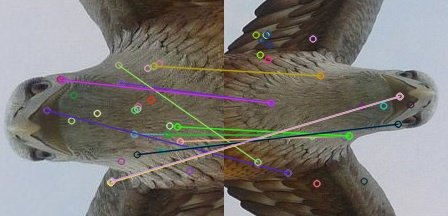
\includegraphics[width=8cm]{Bilder/ZielsetzungUndVorgehensweise/1428488468101951.jpg}
\caption[Beispiel für das Finden von falschen Paaren mit dem DescriptorMatcher von OpenCV]{Beispiel für das Finden von falschen Paaren mit dom DescriptorMatcher von OpenCV\protect\footnotemark}
\label{fig:DescriptorMatcherWrong}
\end{figure}
\footnotetext{\cite{DescriptorMatcherWrong}.}

\noindent Zusätzlich ist die Einwirkung auf den Paarungs- und Suchprozess schwierig, da diese Funktionen von OpenCV stammen, also einer vorgefertigten Bibliothek. Aus diesem Grund wurde auf die Verwendung von Image Targets verzichtet. Anstelle von Image Targets sollten nun mit sogenannten ArUco Markern (\acs{s} \acs{abb} \ref{fig:MarkerExample}) gearbeitet werden. ArUco Marker bilden binäre Bitmasken, die ein eigenständiges Detektieren ermöglichen, da keine aufwendigen Bildmerkmale gesucht werden müssen, sondern fest definierte binäre Bildinformationen.

Vor der Kernentwicklung wurde zuerst eine Recherche nach essentiellen Quellen betrieben, um einen ersten Blick zu erhalten, wie die Detektion von ArUco Markern realisiert werden könnte. Die wichtigsten Quellen, die im Rahmen der Recherche gefunden wurden, bilden das Buch \glqq Mastering OpenCV with Practical Computer Vision Projects\grqq \footcite{Baggioonline} von Daniel Lélis Baggio, die auf OpenCV basierende Bibliothek \glqq ArUco\grqq \footcite{arucoonline} und die Videoreihe \glqq OpenCV Basics\grqq{} zur Kamerakalibrierung mit OpenCV von George Lecakes auf Youtube\footcite{LecakesOpenCV}. Anstelle die externe Bibliothek ArUco zu nutzen, wurde innerhalb der Recherche evaluiert, welche Bestandteile der Bibliothek für einen eigenen Suchalgorithmus verwendet werden könnte. Der Grund für die Entscheidung bildet die bessere Kontrolle einzelner Prozessschritte. Im Vergleich zum Image Target-Ansatz wäre die Detektion von Markern kontrollierbarer und folglich die Problembehandlung simpler. Zusätzlich wäre die einfache Anwendung einer externen Bibliothek, anstelle der selbständigen Entwicklung, fernab des Ziels dieses Praktikums. Eine selbständige Entwicklung stärkt das Verständnis für Anwendungen, die eine externe Bibliothek anbietet.

Für die Darstellung und das Rendern von virtuellen 3D-Objekten wurde OpenGL verwendet. Aus zeitkritischen Gründen musste die Entscheidung gefällt werden, dass sämtliche 3D-Objekte als Kugeln \acs{bzw} Bälle dargestellt werden weil hierdurch eine sehr einfache Kollisionserkennung möglich ist, die für das Einsammeln von Münzen benötigt wird. Dargestellte Bälle unterscheiden sich semantisch in der Farbe:

\begin{itemize}[label=]
    \item Grün:\hspace{0.8cm}Steuerbarer Ball des Spielers
    \item Gelb:\hspace{0.85cm}Bälle, die eingesammelt werden müssen (Münze)
    \item Rot:\hspace{1.0cm}Bälle, die nicht mit dem grünen Ball berührt werden dürfen (Hindernisse)
\end{itemize}

\noindent Bei aufwendigeren Objekten wäre die Verwendung von Bounding Boxes nötig gewesen, um eine Kollisionserkennung realisieren zu können. Dieser Ansatz war nichtsdestotrotz aus zeitkritischen Gründen nicht mehr realisierbar gewesen. Im Rahmen der Implementierung der Kollisionserkennung traten zusätzliche Komplikationen auf, die eine Realisierung des Features nicht ermöglichten. Sämtliche Gründe und Informationen werden im \acs{abs} \ref{kollitionerkennungnnnn} näher erläutert.

Als Versionsverwaltung und Repository wurde GitHub\footnote{Das Projekt ist unter https://github.com/aoezd/Virtual-Reality-Praktikum aufrufbar.} verwendet.


\newpage